\documentclass{standalone}
\usepackage[utf8]{inputenc}

\usepackage{stix2}
\usepackage{cabin}
\usepackage{graphicx}
\usepackage{tikz}
\tikzstyle{every picture}+=[remember picture]
\usetikzlibrary{calc,shapes.multipart,arrows.meta,fit,shapes.arrows,shapes.geometric}
\tikzset{letriangle/.style={regular polygon,regular polygon sides=3,rounded corners=0.5pt,inner sep=0pt,minimum size=2.7mm,outer sep=0mm}}

\newcommand*{\toleft}{\tikz[baseline=-0.6ex]{\node[text width=,letriangle,rotate=90,fill,scale=0.75]{};}}
\newcommand*{\toright}{\tikz[baseline=-0.6ex]{\node[text width=,letriangle,rotate=-90,fill,scale=0.75]{};}}
\newcommand*{\todown}{\tikz[baseline=-1.2ex]{\node[text width=,letriangle,rotate=180,fill,scale=0.75]{};}}
\newcommand*{\toup}{\tikz[baseline=-0.5ex]{\node[text width=,letriangle,fill,scale=0.75]{};}}

\begin{document}
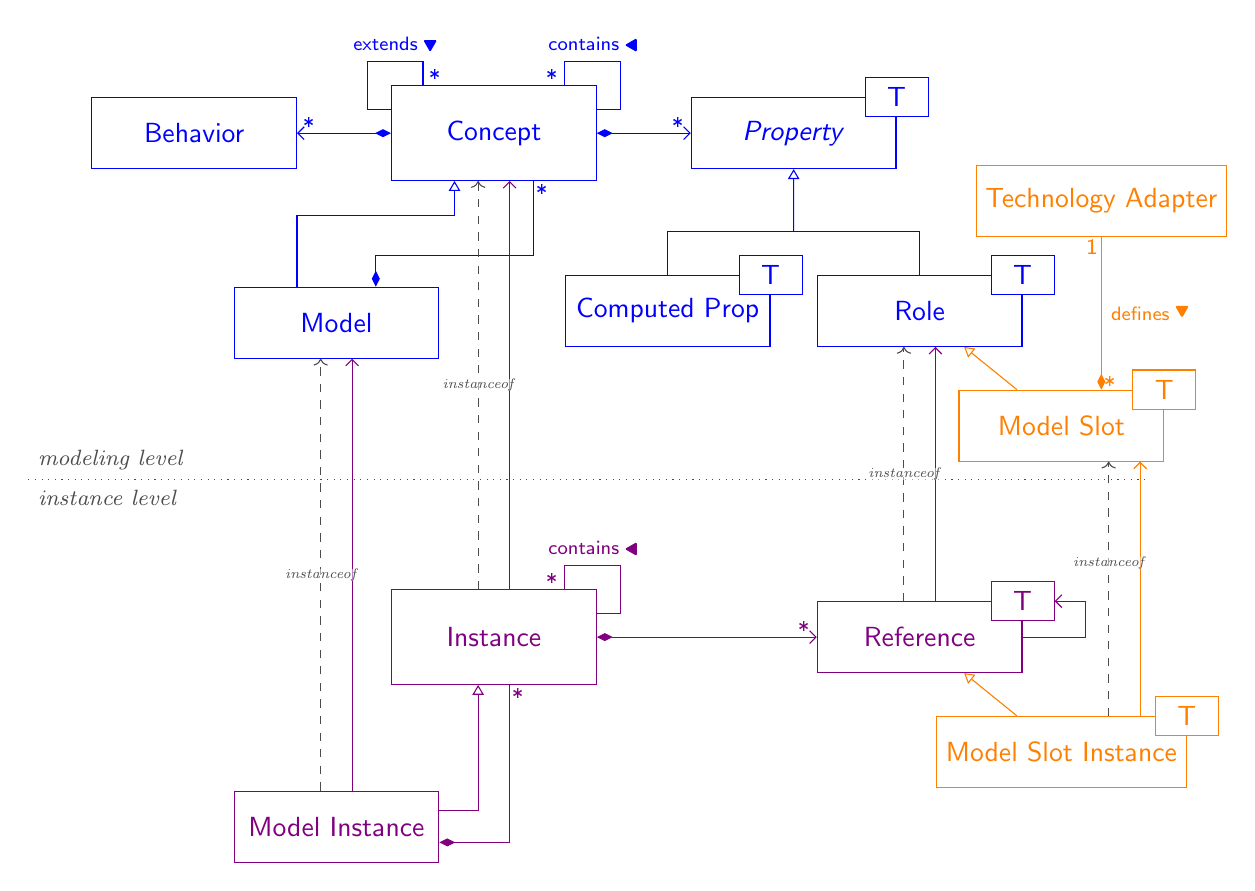
\begin{tikzpicture}[font=\sf,
  class/.style={anchor=center,minimum height=9mm,minimum width=2.6cm},
  iof/.style={font=\tiny\itshape,fill=white,fill opacity=0.5,text opacity=1,inner sep=0pt}]
  \begin{scope}[blue]
    \node[draw,class,minimum height=12mm] (conc)  {Concept};
    \node[draw,class] (vm) at ([xshift=-2cm,yshift=-1.8cm]conc.south) {Model};
    \node[draw,class,right=2.5cm] (prop) at (conc) {\textit{Property}};
    \node[draw,class,left=2.5cm] (beh) at (conc) {Behavior};
    \node[draw,class] (role) at ([yshift=-1.8cm,xshift=1.6cm]prop.south) {Role};
    \node[draw,class] (cprop) at ([yshift=-1.8cm,xshift=-1.6cm]prop.south) {Computed Prop};
    \node[draw,anchor=center,minimum height=5mm,minimum width=0.8cm,fill=white] (propparam) at (prop.north east) {T};
    \node[draw,anchor=center,minimum height=5mm,minimum width=0.8cm,fill=white] (roleparam) at (role.north east) {T};
    \node[draw,anchor=center,minimum height=5mm,minimum width=0.8cm,fill=white] (cpropparam) at (cprop.north east) {T};
    \node[coordinate] (middle) at (barycentric cs:prop=1.6,cprop=1 ,role=1) {};
    % \node[draw,class,blue] (ms) at ([yshift=-1.8cm]vm.south) {ModelSlot};
    % \node[draw=blue,class,right=1.8cm] (mstype) at (ms.east) {\color{orange}MSType};
    % \node[draw,class,right=1.8cm,blue] (action) at (vm.east) {Action};
    % \node[draw=blue,class] (taconc)  {\color{orange}TAConcept};
    % \node[draw,class,right=4.2cm,blue] (ta) at (crole.east) {TechnologyAdapter};
    % 
    \draw[{Straight Barb}-Diamond] (prop) -- (conc) node[pos=0,above left,inner sep=2pt,font=\footnotesize\sf] {\textasteriskcentered};
    % 
    \coordinate[above left=3mm] (p) at (conc.north west);
    \draw ([yshift=3mm]conc.west) -| (p) -| ([xshift=-9mm]conc.north) node[pos=0.25,above,font=\scriptsize\sf] {extends\hspace{2pt}\todown} node[pos=1,above right,inner sep=2pt,font=\footnotesize\sf] {\textasteriskcentered};
    \coordinate[above right=3mm] (p2) at (conc.north east);
    \draw ([yshift=3mm]conc.east) -| (p2) -| ([xshift=9mm]conc.north) node[pos=0.25,above,font=\scriptsize\sf] {contains\hspace{2pt}\toleft} node[pos=1,above left,inner sep=2pt,font=\footnotesize\sf] {\textasteriskcentered};
    % 
    % \draw (crole) -| ([yshift=-1.5mm]barycentric cs:crole=1,conc=1) node[coordinate] (m1) {} node[pos=0,above left,inner sep=1pt,font=\footnotesize\sf] {\textasteriskcentered};
    \draw[{Straight Barb}-Diamond] (beh) -- (conc) node[pos=0,above right,inner sep=2pt,font=\footnotesize\sf] {\textasteriskcentered};
    \draw[-{Triangle[open]}] ([xshift=-5mm]vm.north) -- +(0,0.9) -| ([xshift=-5mm]conc.south) ;
    \draw[Diamond-] ([xshift=5mm]vm.north) -- +(0,0.4) -| ([xshift=5mm]conc.south) node[pos=1,below right,inner sep=1pt,font=\footnotesize\sf] {\textasteriskcentered};
    \draw[-{Triangle[open]}] (middle) -- (prop) ;
    \draw (role) |- (middle) ;
    \draw (cprop) |- (middle) ;
  \end{scope}

  \begin{scope}[yshift=-6.4cm]
    \begin{scope}[violet]
      \node[draw,class,minimum height=12mm] (inst)  {Instance};
      \node[draw,class] (vmi) at ([xshift=-2cm,yshift=-1.8cm]inst.south) {Model Instance};
%      \node[draw,class] (val) at (inst.north east-|prop) {Value};
      \node[draw,class] (ref) at (inst-|role) {Reference};
      \node[draw,anchor=center,minimum height=5mm,minimum width=0.8cm,fill=white] (refparam) at (ref.north east) {T};
      %
      \draw[{Straight Barb}-Diamond] (ref) -- (inst) node[pos=0,above left,inner sep=2pt,font=\footnotesize\sf] {\textasteriskcentered};
%      \draw[{Straight Barb}-Diamond] (val.west) -- ([yshift=1.5mm]inst.east) node[pos=0,above left,inner sep=2pt,font=\footnotesize\sf] {\textasteriskcentered};
      \draw[Diamond-] ([yshift=-2mm]vmi.east) -| ([xshift=2mm]inst.south) node[pos=1,below right,inner sep=1pt,font=\footnotesize\sf]{\textasteriskcentered};
      \draw[-{Triangle[open]}] ([yshift=2mm]vmi.east) -| ([xshift=-2mm]inst.south) ;
      \coordinate[above right=3mm] (p2) at (inst.north east);
      \draw ([yshift=3mm]inst.east) -| (p2) -| ([xshift=9mm]inst.north) node[pos=0.25,above,font=\scriptsize\sf] {contains\hspace{2pt}\toleft} node[pos=1,above left,inner sep=2pt,font=\footnotesize\sf] {\textasteriskcentered};
      \draw[-Straight Barb] ([xshift=2mm]inst.north) -- ([xshift=2mm]conc.south);
      \draw[-Straight Barb] ([xshift=2mm]vmi.north) -- ([xshift=2mm]vm.south);
      \draw[-Straight Barb] ([xshift=2mm]ref.north) -- ([xshift=2mm]role.south);
      \draw[-Straight Barb] (ref.east) -- +(0.8,0) |- (refparam.east) node[pos=0,coordinate] (a) {};
%      \draw[-Straight Barb] (val.north) -- (prop.south);
    \end{scope}
  \end{scope}

  \begin{scope}[orange]
    \node[draw,class] (ms) at ([yshift=-1cm,xshift=1.8cm]role.south) {Model Slot};
    \node[draw,anchor=center,minimum height=5mm,minimum width=0.8cm,fill=white] (msparam) at (ms.north east) {T};
    \draw[-{Triangle[open]}] (ms) -- (role) ;
    \node[draw,class] (msi) at ([yshift=-1cm,xshift=1.8cm]ref.south) {Model Slot Instance};
    \node[draw,anchor=center,minimum height=5mm,minimum width=0.8cm,fill=white] (msiparam) at (msi.north east) {T};
    \draw[-{Triangle[open]}] (msi) -- (ref) ;
    \draw[-Straight Barb] ([xshift=10mm]msi.north) -- ([xshift=10mm]ms.south);
    \node[draw,class] (ta) at ([xshift=1cm,yshift=1.4cm]role.east) {Technology Adapter};
    \draw[Diamond-] (ms.north-|ta) -- node[right,font=\scriptsize\sf] {defines\hspace{2pt}\todown} (ta) node[pos=1,below left,inner sep=1pt,font=\footnotesize\sf]{1} node[pos=0,above right,inner sep=1pt,font=\footnotesize\sf]{\textasteriskcentered};
  \end{scope}

  \begin{scope}[black!70]
    \node[coordinate] (middle) at ($(vm)!0.5!(inst)$) {};
    \node[coordinate] (left) at (beh.west|-middle) {};
    \node[coordinate] (right) at (a|-middle) {};
    \begin{scope}[font=\footnotesize\itshape]
      \draw[dotted] ([xshift=-8mm]left) -- ([xshift=8mm]right) node[pos=0,above right] {modeling level} node[pos=0,below right] {instance level};
    \end{scope}
    \begin{scope}[dashed,->]
      \draw ([xshift=-2mm]inst.north) -- node[iof] {instanceof} ([xshift=-2mm]conc.south);
      \draw ([xshift=-2mm]vmi.north) -- node[iof] {instanceof} ([xshift=-2mm]vm.south);
      \draw ([xshift=-2mm]ref.north) -- node[iof] {instanceof} ([xshift=-2mm]role.south);
      \draw ([xshift=6mm]msi.north) -- node[pos=0.6,iof] {instanceof} ([xshift=6mm]ms.south);
    \end{scope}
  \end{scope}


\end{tikzpicture}

\end{document}
